%This chapters purpose is to link general relativity to a basic michelson interferometer. I will keep the general relativity to a minimum, since this isn't a textbook on GR, however there is a small amount required to know why gravitational wave detectors are so big, why they are L shaped, etc. It will then expand on the basic michelson by adding the cavities. This is a good point to link sources to the detector, since the signal recycling adds shaping, its good to know why we aimed for 100Hz (I actually don't know why this was done, for some reason LIGO is optimised for detecting heavy black holes I think). Talk about noise sources, noise and senstivity curves, transfer functions between differential arm motion to light modulation at the AS port, mention the standard quantum limit. A detailed explanation of shot noise and radiation pressure noise should be in here, since these basically give you the requirements for the laser chapter and the photodiode chapter. Once the noise sources are covered, the BNS range can be shown. It makes sense to introduce the current detectors in more detail, and then talk about the 3rd generation of detectors. More novel topologies can be mentioned after. 
\section{Introduction}
The aim of this chapter is to outline some things about our universe we would like to know, how a gravitation wave allows this to be known, how an interferometer can be used to measure gravitational waves, the fundemental noise sources these detectors face. These noise sources can be reduced by making changes to the readout of the LIGO detector and by building new interferometers that use new technology. In this thesis, power of the laser and BHD is explored. Third generation detectors may operate at 2um, and so 2um detectors were characterised.
\section{Measuring Gravitational Waves}
\paragraph{general relativity (L shaped IFO)}
\paragraph{sources of GW}
\paragraph{observation runs and discoveries (detector hierarchy)}
\paragraph{The need for increasing detections...}
\section{Sources of noise when detecting gravitational waves}
\paragraph{shot noise and laser power}
\paragraph{quantum efficiency}
\paragraph{power recycling}
\paragraph{signal recycling to shape quantum noise}
\paragraph{squeezed light}
\paragraph{frequency dependent squeezing}
\paragraph{radiation pressure noise?}
\paragraph{other topologies of detectors}
\paragraph{other noise sources}
\section{The future of gravitational wave detectors}
\paragraph{cyro}
\paragraph{silicon}
\paragraph{2um or 1550}
\section{conclusion}
\begin{figure}
	\centering
	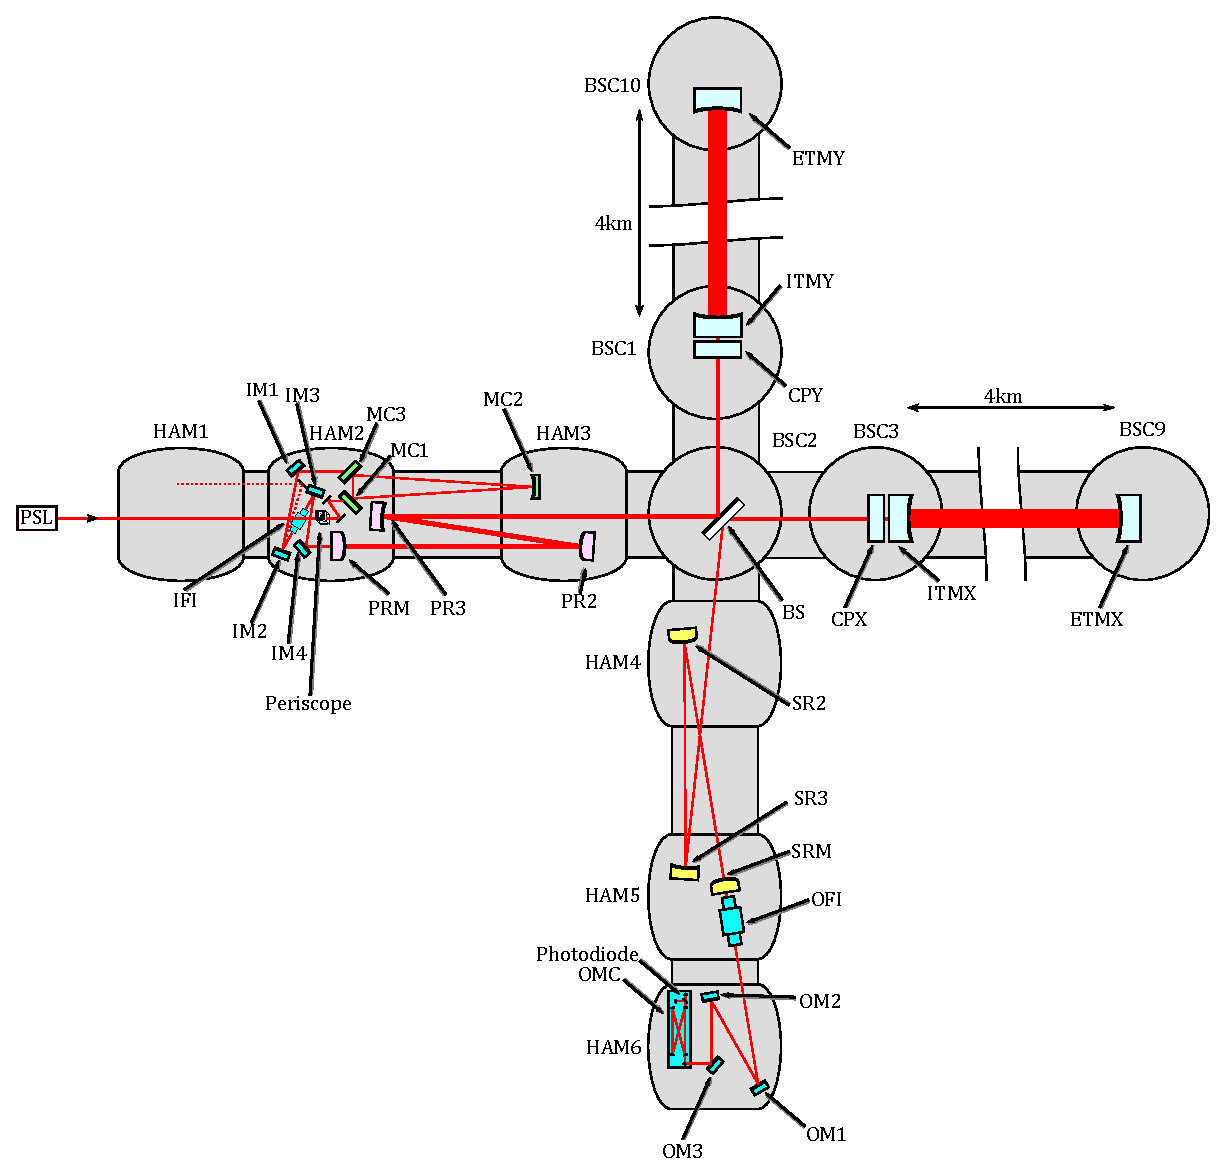
\includegraphics[width=1\linewidth]{Figures/LIGO_layout}
	\caption{}
	\label{fig:ligolayout}
\end{figure}
